\documentclass[a4paper, 12pt]{report}

\usepackage[utf8]{inputenc}
\usepackage[french]{babel}
%\usepackage[english]{babel}
\usepackage[T1]{fontenc}
% \usepackage[latin1]{inputenc}

\usepackage[top=3cm, bottom=3cm, left=2.3cm,right=2cm]{geometry}
\usepackage{graphicx}
\usepackage{color}
\usepackage{titlepic}
\usepackage{hyperref}
%\usepackage{url}
\usepackage[table]{xcolor}
\usepackage{tipa} % phonétique
\definecolor{light-gray}{gray}{0.50}
\definecolor{very-light-gray}{gray}{0.9}

\usepackage{listings}
\lstset{language=python, 
  basicstyle=\scriptsize, 
  numbers=left,
  numberstyle=\tiny\color{light-gray},  % the style that is used for the line-numbers
  numbersep=5pt,                  % how far the line-numbers are from the code
  backgroundcolor=\color{white},      % choose the background color. You must add \usepackage{color}
  showspaces=false,               % show spaces adding particular underscores
  showstringspaces=false,         % underline spaces within strings
  showtabs=false,                 % show tabs within strings adding particular underscores
  frame=single,                   % adds a frame around the code
  %rulecolor=\color{black},        % if not set, the frame-color may be changed on line-breaks within not-black text (e.g. commens (green here))
  tabsize=4,                      % sets default tabsize to 2 spaces
  captionpos=b,                   % sets the caption-position to bottom
  breaklines=true,                % sets automatic line breaking
  breakatwhitespace=false,        % sets if automatic breaks should only happen at whitespace
  title=\lstname,                   % show the filename of files included with \lstinputlisting;
                                  % also try caption instead of title
  %keywordstyle=\color{blue},          % keyword style
  commentstyle=\color{light-gray},       % comment style
  %stringstyle=\color{yellow}         % string literal style
}

%en-tete de page
\usepackage{fancyhdr}
\lhead{HumanTech Institute}
\chead{}
\rhead{\today}
\pagestyle{fancy}

%\renewcommand{\thesection}{\arabic{section}} % pour numrotation des sections

\titlepic{
\includegraphics[width=1\textwidth]{img/humantechlogo.jpg}}
\title{\huge{HES-SO} \\ \Huge{\textbf{\textsc{HumanTech}}} \\
\vspace{2cm} \huge{\textbf{Manuel}} \\ 
\huge{Installation d'un serveur ownCloud sur SWITCHengines}}
\author{\\ \\ Jacky \textsc{Casas} \\
\\ \\
Julien \textsc{Tscherrig} \\
Omar \textsc{Abou Khaled} \\
\\
\footnotesize{Version 1}}
\date{\today}


\begin{document}
\maketitle % page de garde
\newpage

%\setcounter{tocdepth}{1} % limit the table of contents to depth 1
\tableofcontents
\newpage

%\chapter{Introduction}
%\section{Introduction}

\chapter{SWITCHengines}
\section{Création d'un compte sur SWITCHengines}

Toute personne qui possède un compte AAI chez SWITCH (SWITCHaai) peut créer un compte sur SWITCHengines, le cloud privé de SWITCH. Pour ce faire, il faut aller à l'adresse \url{https://cloud-id.switch.ch/}. Vous serez redirigé vers une page de connexion AAI standard (figure \ref{loginAAI}a). Il vous faudra alors sélectionner l'école dans laquelle vous êtes enregistré puis entrer votre nom d'utilisateur et mot de passe (figure \ref{loginAAI}b).

\begin{figure}[h!]
    \centering
    \begin{tabular}{cc}
      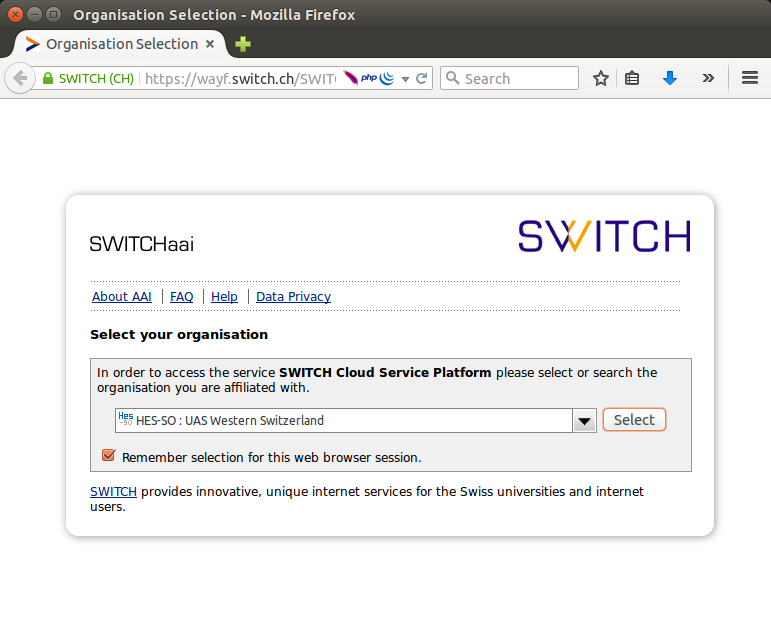
\includegraphics[width=.48\linewidth]{img/switch1.png} &
      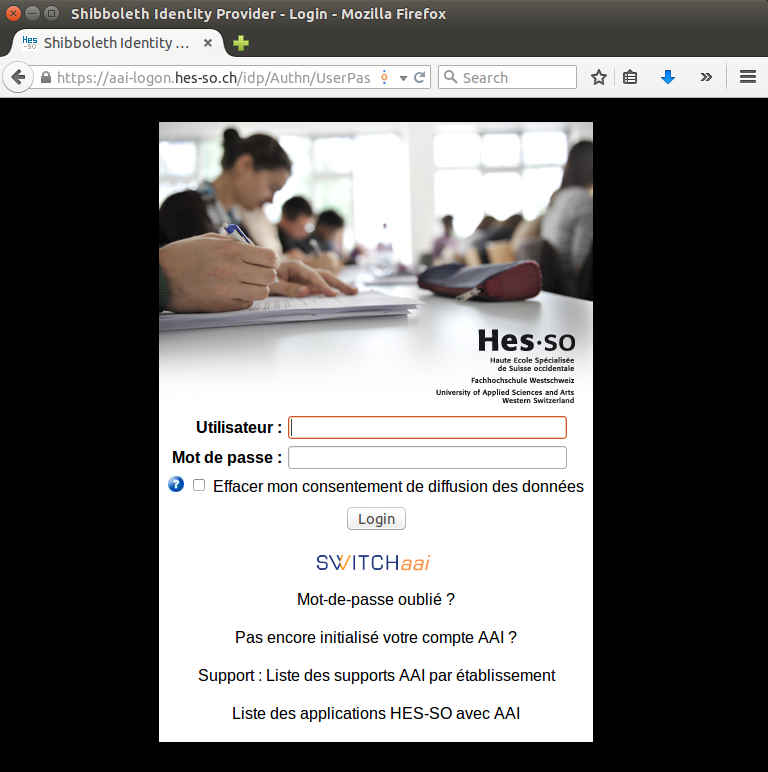
\includegraphics[width=.48\linewidth]{img/switch2.png} \\
      (a) & (b)\\
    \end{tabular}
    \caption{Connexion AAI (a) Ecole (b) Utilisateur et mot de passe
    \label{loginAAI}}
\end{figure}

Une fois connecté, vous arriverez sur une page qui vous propose de créer un compte pour pouvoir accéder au Cloud Service de SWITCH (figure \ref{loginEngines}a). Cliquez donc sur le lien prévu à cet effet. On vous demandera alors de choisir un mot de passe (figure \ref{loginEngines}b).

\begin{figure}[h!]
    \centering
    \begin{tabular}{cc}
      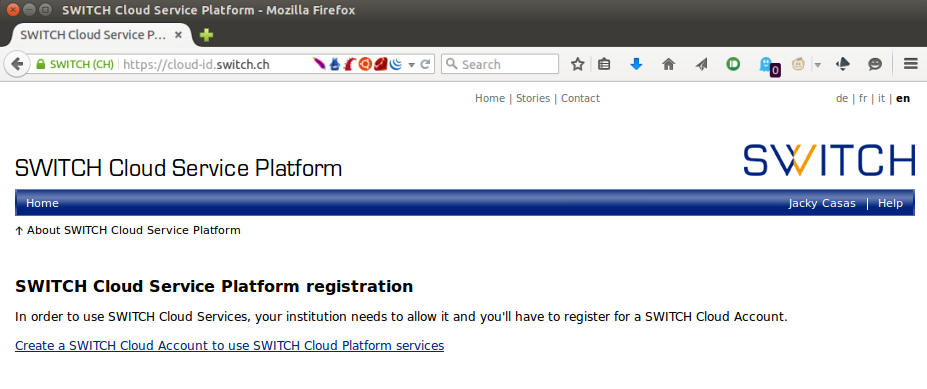
\includegraphics[width=.48\linewidth]{img/switch3.png} &
      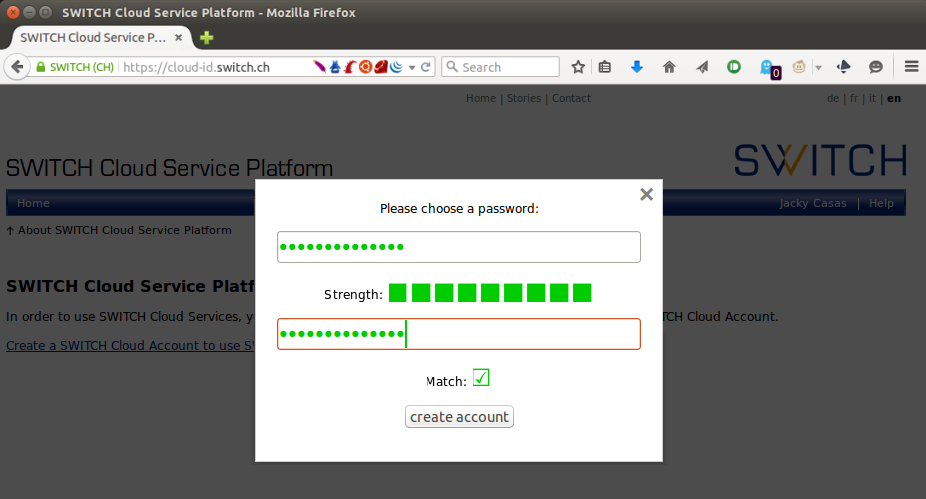
\includegraphics[width=.48\linewidth]{img/switch4.png} \\
      (a) & (b)\\
    \end{tabular}
    \caption{Création du compte Cloud Service (a) Accueil (b) Choix du mot de passe
    \label{loginEngines}}
\end{figure}

Vous arrivez ensuite sur une page récapitulative qui vous indique votre identifiant (attention, il peut être différent de votre identifiant AAI). Et en dessous vous voyez les différents services auxquels vous avez accès. Vous pouvez voir cette page à la figure \ref{enginesRecap}.

\begin{figure}[h]
  \centering
    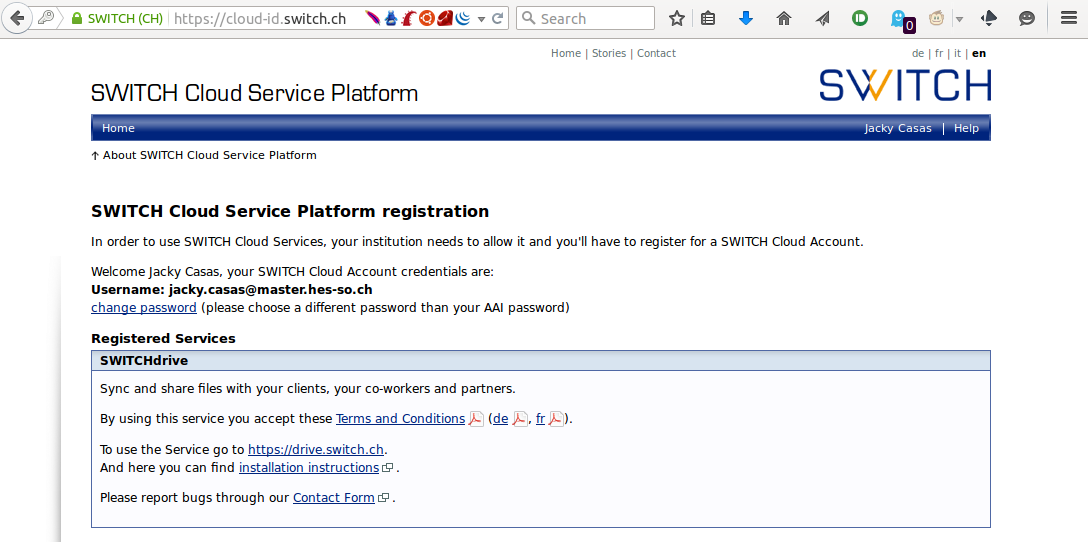
\includegraphics[width=\linewidth]{img/switch5.png}
  \caption{Récapitulatif, informations de votre compte}
  \label{enginesRecap}
\end{figure}

Sur cette figure, nous voyons que nous avons accès à SWITCHdrive (dans l'encadré), mais pas à SWITCHengines. Pour y avoir accès, il faut demander un accès en envoyant un e-mail à engines-support@switch.ch. Cette métodologie est valabe au moment de la rédaction de ce document. C'est pour faire partie de la phase pilote qui dure jusqu'à fin juin 2015.

%--> Users from academic can start using SWITCHengines as test users in the pilot phase of SWITCHengines. The pilot phase lasts until end of June 2015. Apply for an account on engines-support@switch.ch.
%\url{http://projects.switch.ch/scale/}

Vous recevrez un code d'activation par e-mail. Vous aurez ensuite accès à SWITCHengines, comme on le voit sur la figure \ref{enginesRecap2}.

\begin{figure}[h]
  \centering
    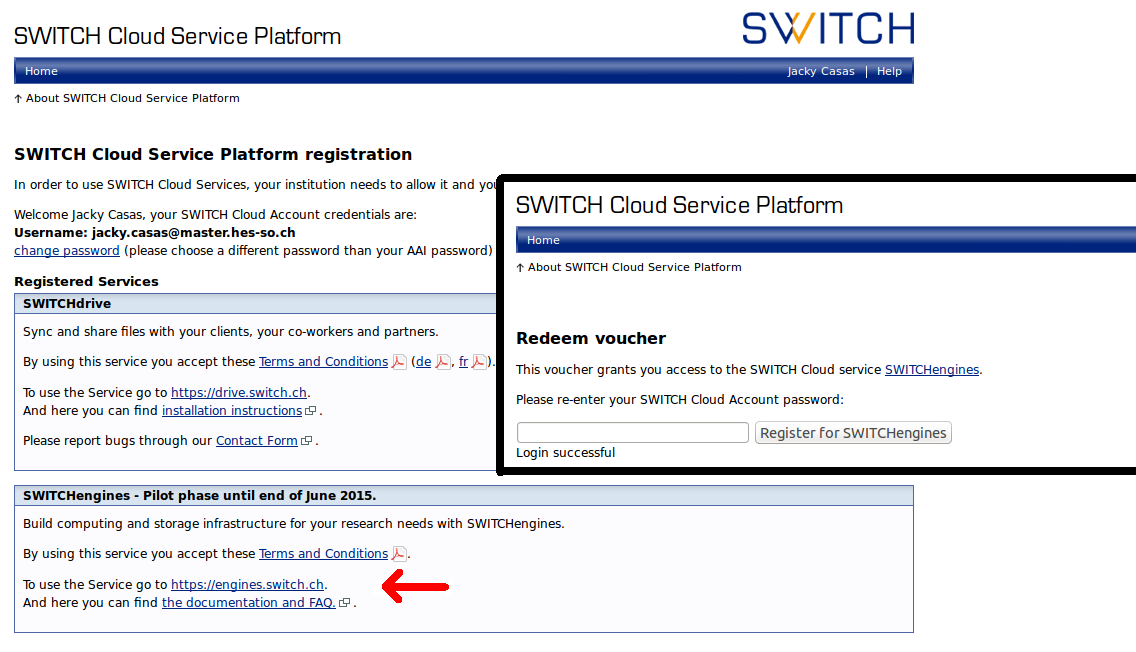
\includegraphics[width=\linewidth]{img/switch6.png}
  \caption{Accès à SWITCHengines et code d'activation}
  \label{enginesRecap2}
\end{figure}

\clearpage


%---------------------------------------------------------------------------------------------------------------------------------
\section{Connexion à SWITCHengines}


Si votre compte est configuré pour accéder à SWITCHengines, vous pouvez maintenant aller à l'adresse \url{https://engines.switch.ch/horizon} qui est la page de connexion (figure \ref{loginSWITCHengines}), et vous loguer.

\begin{figure}[h]
  \centering
    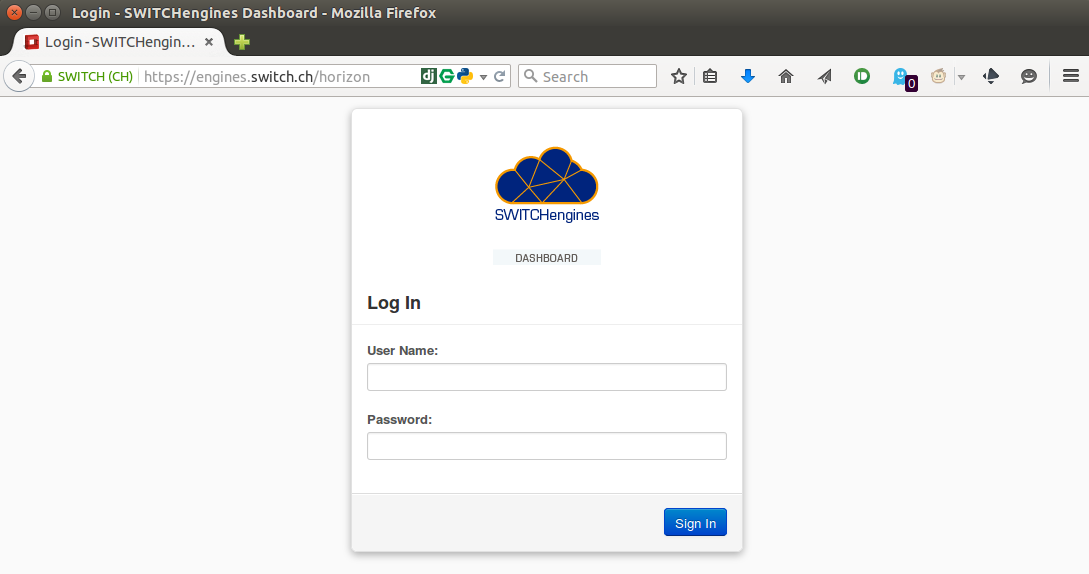
\includegraphics[width=\linewidth]{img/engines1.png}
  \caption{Page de connexion à SWITCHengines}
  \label{loginSWITCHengines}
\end{figure}

Vous arrivez ensuite sur le dashboard de SWITCHengines (figure \ref{dashboard1}). On voit sur l'image qu'aucune instance n'est pour l'instant créée. On va donc en créer une. 

\begin{figure}[h]
  \centering
    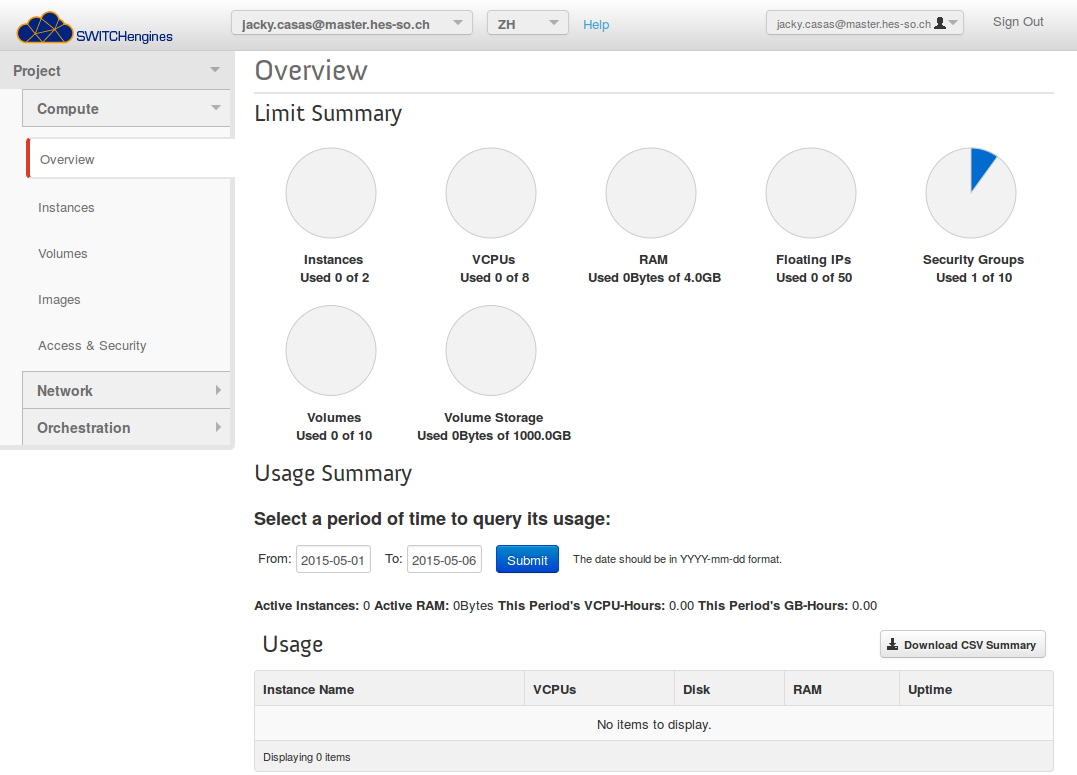
\includegraphics[width=\linewidth]{img/dashboard1.png}
  \caption{Dashboard de SWITCHengines}
  \label{dashboard1}
\end{figure}

\clearpage


%---------------------------------------------------------------------------------------------------------------------------------
\section{Création d'une instance}

\subsection{Choix de la zone}

Tout au sommet du dashboard se trouve un petit menu déroulant qui contient « ZH » et « LS ». Cela correspond à « Zürich » et « Lausanne ». Ce sont les deux zones disponibles, elles correspondent aux lieux où se trouvent les datacenters. Il faut choisir où on veut lancer notre instance avant de commencer.

\subsection{Création d'une paire de clés}

\begin{enumerate}
 \item Cliquer sur « Access \& Security » dans le menu de gauche.
 \item Cliquer sur l'onlet « Key Pairs ».
 \item Cliquer sur « + Create Key Pair ».
 \item Donner un nom à sa paire de clés.
 \item Télécharger le fichier .pem qui est la clé privée. Elle sera utilisée pour accéder aux instances créées.
\end{enumerate}


\subsection{Création d'un Security Group}

\begin{enumerate}
 \item Cliquer sur « Access \& Security » dans le menu de gauche.
 \item Cliquer sur le bouton « Manage Rules » à droite du Security Group par défaut. Cela va permettre d'éditer les règles d'accès.
 \item Cliquer sur « + Add Rule » pour ajouter une nouvelle règle.
 \item Choisir « SSH » dans le menu déroulant. Les champs suivants peuvent être laissés à leurs valeurs par défaut. Mais attention, si le CIDR est à 0.0.0.0/0, cela veut dire qu'on peut accéder à l'instance depuis n'importe où. Selon le but de l'instance, il faudrait limiter l'accès pour des raisons de sécurité.
 \item Cliquer sur « Add »  pour ajouter la règle. Nous pourrons donc accéder aux instances qui sont dans le Security Group par défaut par SSH.
\end{enumerate}

\noindent NB : pour pouvoir accéder à l'instance par HTTP ou HTTPS, il faut procéder de la même manière que pour ajouter la règle pour le SSH.
      
    
\subsection{Lancer une instance}

\begin{enumerate}
 \item Cliquer sur « Instances » dans le menu de gauche.
 \item Cliquer sur « Launch instance » en haut à droite.
 \item Donner un nom à l'instance, comme par exemple « owncloudserver ».
 \item Choisir la taille de l'instance, par exemple « c1.small ».
 \item Entrer 1 dans le nombre d'instance à lancer.
 \item Sélectionner « Boot from image » pour utiliser une image déjà existante d'un système d'exploitation.
 \item Choisir le système d'exploitation, par exemple « Ubuntu Trusty 14.04 (SWITCHengines) (1.5 GB) » pour une instance Ubuntu.
 \item Cliquer sur l'onglet « Access \& Security » et sélectionner la keypair créée précédemment
 \item Cliquer sur l'onglet « Networking » et sélectionner le réseau « private » (drag \& drop).
 \item Cliquer sur « Launch » en-bas à droite pour lancer l'instance. 
\end{enumerate}
    
\begin{figure}[h]
  \centering
    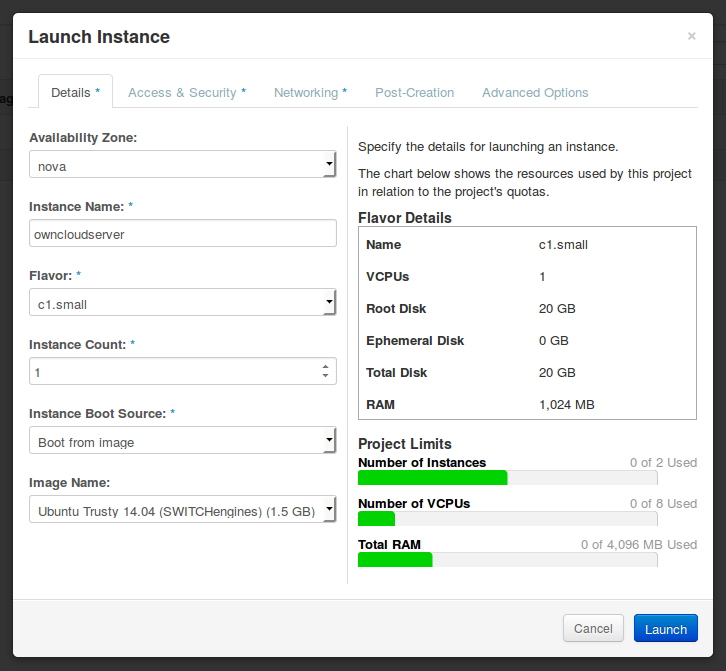
\includegraphics[width=0.7\linewidth]{img/instanceCreation1.png}
  \caption{Paramètres pour créer l'instance}
  \label{instanceCreation1}
\end{figure}

Si tout se passe bien, l'instance se lancer et elle est prête au bout de quelques secondes. Si au contraire ça ne fonctionne pas, il faut faire un tour sur les pages d'aide : \\
\url{https://help.switch.ch/engines}.

\subsection{Attribuer une IP flottante à l'instance}

Pour que l'instance ait une adresse IP accessible depuis internet (et pas uniquement depuis l'intérieur du cloud), il faut lui attribuer une IP. Pour ce faire, il faut aller à l'endroit où les instances sont listées et cliquer sur le bouton « More » (fig. \ref{instanceIP} point 1) puis « Associate Floating IP » (fig. \ref{instanceIP} point 2). Une fenêtre s'ouvre, vous devez sélectionner une IP. Si vous n'en avez pas, cliquer sur le petit « + » pour qu'une IP vous soit attribuée. Vous sélectionnez le port et cliquez sur « Associate ». Sur la liste des instances, vous pouvez maintenant voir que votre instance a une IP externe (fig. \ref{instanceIP} point 3).

\begin{figure}[h]
  \centering
    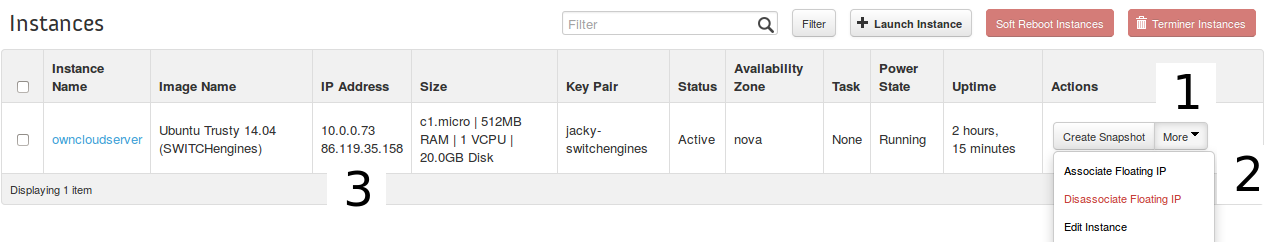
\includegraphics[width=\linewidth]{img/instanceIP.png}
  \caption{Etapes d'ajout d'une IP externe}
  \label{instanceIP}
\end{figure}

\subsection{Se connecter à l'instance}

Une fois l'instance lancée et l'IP attribuée, il est possible de se connecter à l'instance via SSH. Il faut aller à l'endroit où se trouve la clé privée précédemment créée et écrire la commande : ``\texttt{ssh -i <keypair.pem> <username>@<public IP>}'', où \texttt{<keypair.pem>} est la clé privée, \texttt{<username>} est le nom d'utilisateur créé pour l'instance (pour une instance ubuntu, le nom d'utilisateur est \texttt{ubuntu}, pour une instance CentOS, le nom d'utilisateur est \texttt{admin}) et \texttt{<public IP>} est l'IP public qu'on vient d'attribuer (dans ce cas, 86.119.35.158). \\

NB : si l'accès est refusé, c'est parce que les droits sur la clé privée sont trop laxistes, il faut donc restraintre les droits de cette manière : ``\texttt{sudo chmod 600 <keypair.pem>}'' 

NB2 : si ça ne fonctionne toujours pas, précédez la commande de connexion par ``\texttt{sudo}''

\vspace{0.6cm}
Voici la situation d'une connexion depuis un terminal standard :

\vspace{0.4cm}
\begin{lstlisting}[language=bash]
  jacky@grid:~$ ssh -i jacky-switchengines.pem ubuntu@86.119.35.158 
  Welcome to Ubuntu 14.04.2 LTS (GNU/Linux 3.13.0-48-generic x86_64)

  * Documentation:  https://help.ubuntu.com/

    System information as of Thu May 21 13:07:10 CEST 2015

    System load: 0.16              Memory usage: 10%   Processes:       51
    Usage of /:  65.5% of 1.30GB   Swap usage:   0%    Users logged in: 0

    Graph this data and manage this system at:
      https://landscape.canonical.com/

    Get cloud support with Ubuntu Advantage Cloud Guest:
      http://www.ubuntu.com/business/services/cloud

  0 packages can be updated.
  0 updates are security updates.


  The programs included with the Ubuntu system are free software;
  the exact distribution terms for each program are described in the
  individual files in /usr/share/doc/*/copyright.

  Ubuntu comes with ABSOLUTELY NO WARRANTY, to the extent permitted by
  applicable law.

  ubuntu@owncloudserver:~$
\end{lstlisting}

Pour se déconnecter de l'instance, il suffit juste d'écrire ``\texttt{exit}'' dans la console.

\chapter{ownCloud}
%---------------------------------------------------------------------------------------------------------------------------------
\section{Introduction}

\noindent Un serveur ownCloud peut être installé de différentes façons \footnote{\url{https://owncloud.org/install/\#instructions-server}} :

\begin{enumerate}
 \item Par le gestionnaire de package de votre système (ex : apt-get)
 \item En lançant une image cloud déjà configurée (disponible sur Azure, Google Cloud, Amazon AWS, Juju)
 \item Avec un web installer (fichier PHP à télécharger)
 \item Avec l'archive d'ownCloud
\end{enumerate}


Nous allons utiliser ici la quatrième façon, c'est-à-dire une installation depuis l'archive officielle d'ownCloud. Cette technique nous permet d'être plus libre, de pouvoir gérer soit-même les mises à jour et de modifier le code source si nécessaire. Par contre il y a des inconvénients. Nous avons l'obligation de tout installer depuis zéro (services, base de données, serveur, réseau, autorisations, etc.).

Nous allons à présent pouvoir installer ownCloud serveur sur notre instance. La procédure expliquée ci-bas est tirée de la page suivante : 
\url{https://doc.owncloud.org/server/8.0/admin_manual/installation/source_installation.html}. Il s'agit du manuel d'installation d'ownCloud Sever 8.

%---------------------------------------------------------------------------------------------------------------------------------
\section{Installation}

\subsection{Mise à jour des packages de la distribution}

Avant de commencer, il est préférable de mettre à jour la liste des packages disponibles sur votre instance Ubuntu et de mettre à jour les logiciels. Voici les deux commandes à exécuter : \\

\begin{lstlisting}[language=bash]
  sudo apt-get update
  sudo apt-get upgrade
\end{lstlisting}

\subsection{Installation de PHP et MariaDB}

Il faut installer PHP ainsi que la base de données MariaDB : \\

\begin{lstlisting}[language=bash]
  sudo apt-get install apache2 mariadb-server libapache2-mod-php5
  sudo apt-get install php5-gd php5-json php5-mysql php5-curl
  sudo apt-get install php5-intl php5-mcrypt php5-imagick
\end{lstlisting}

Lors de l'installation, l'assistant vous demande si vous voulez vraiment installer les packages, tapez simplement ``Y'' (pour Yes). Ensuite MariaDB demande un mot de passe pour l'utilisateur root. Choisissez-en un et mémorisez-le.


\subsection{Téléchargement de l'archive ownCloud}

Il faut à présent télécharger l'archive ownCloud. Pour cela il y a différentes façon. La première est de suivre de lien \url{https://owncloud.org/install/}, de cliquer sur \texttt{Download} et de télécharger l'archive \texttt{.tar.bz2} ou \texttt{.zip}. Il faudra ensuite envoyer cette archive sur votre instance pour l'utiliser. Dans ce cas, vous accéderez à la dernière version stable d'ownCloud server. La seconde façon est de télécharger l'archive directement depuis votre instance. Il faudra savoir le numéro de version voulue et la remplacer dans le lien ci-dessous. Voici comment le faire : \\

\begin{lstlisting}[language=bash]
  wget https://download.owncloud.org/community/owncloud-8.0.3.tar.bz2
\end{lstlisting}

A partir de là, la stratégie est la même dans les deux cas : il faut désarchiver (dézipper) le fichier : \\

\begin{lstlisting}[language=bash]
  sudo tar -xjvf owncloud-8.0.3.tar.bz2 
\end{lstlisting}

Il faut ensuite copier le dossier \texttt{owncloud} à la racine du serveur Apache : \\

\begin{lstlisting}[language=bash]
  sudo cp -r owncloud /var/www/
\end{lstlisting}

\subsection{Configuration du serveur Apache}

Nous voulons créer un fichier de configuration Apache pour ownCloud, voici la recette : \\

\begin{lstlisting}[language=bash]
  cd /etc/apache2/conf-available/
  sudo touch owncloud.conf
  sudo vim owncloud.conf
\end{lstlisting}

Nous nous trouvons alors dans VIM, il faut écrire les lignes suivantes dans le fichier \texttt{owncloud.conf} : \\

\begin{lstlisting}[language=bash]
  Alias /owncloud /var/www/owncloud
  <Directory /var/www/owncloud/>
     AllowOverride All
     Satisfy Any
  </Directory>
\end{lstlisting}

% s'il y a un WebDAV sur le serveur, il faut le désactiver en ajoutant ``Dav Off'' dans ``<Directory''

Et pour que le fichier soit pris en compte, on ajoute un lien symbolique dans le bon dossier : \\

\begin{lstlisting}[language=bash]
  sudo ln -s /etc/apache2/conf-available/owncloud.conf /etc/apache2/conf-enabled/owncloud.conf
\end{lstlisting}

Il faut également activer le mode \texttt{rewrite} sur Apache (et redémarrer Apache pour que le changement soit pris en compte) : \\

\begin{lstlisting}[language=bash]
  sudo a2enmod rewrite
  service apache2 restart
\end{lstlisting}

% ATTENTION A CA :
  % When using SSL, take special note on the ServerName. 
  % You should specify one in the server configuration, 
  % as well as in the CommonName field of the certificate. 
  % If you want your ownCloud to be reachable via the internet, 
  % then set both of these to the domain you want to reach your ownCloud server.
  
  
Notre serveur Apache est correctement installé. Pour en être sûr, accédez à votre instance par HTTP en insérant l'IP de l'instance dans un navigateur. Attention, pour que ça fonctionne il faut avoir ajouté une règle pour le HTTP dans le \texttt{Security Group} lié à votre instance. Si tout fonctionne, vous verrez la page de la figure \ref{apacheisworking} s'afficher.


\begin{figure}[h]
  \centering
    
\includegraphics[width=\linewidth]{img/apacheIsWorking.png}
  \caption{Page d'accueil du serveur Apache}
  \label{apacheisworking}
\end{figure}

\section{Gestion des droits}

Pour accéder à l'interface web d'ownCloud server, il suffit d'ajoute ``\texttt{/owncloud}`` à la fin de l'IP de l'instance dans le navigateur. A l'état actuel, ownCloud n'a pas les droits corrects pour pouvoir écrire sur le disque comme on peut le voir sur la figure \ref{nowriteaccess}.

\begin{figure}[h]
  \centering
    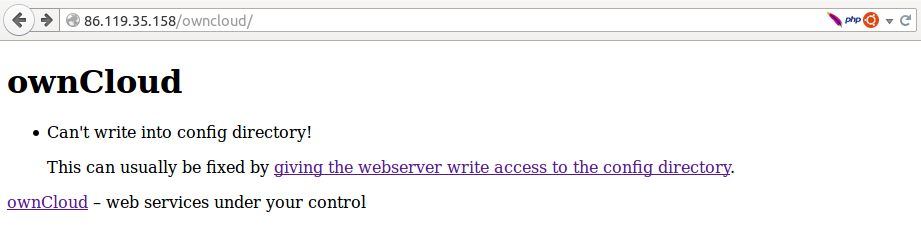
\includegraphics[width=\linewidth]{img/OCWriteAccess.png}
  \caption{OwnCloud n'a pas les droits d'écriture dans le dossier de configuration}
  \label{nowriteaccess}
\end{figure}

Il faut donc que vous lanciez le scipt ci-dessous en mode root après l'avoir déplacé sur l'instance : \texttt{sudo ./changeWriteAccessOC.sh}

\lstinputlisting[language=Python]{code/changeWriteAccessOC.sh}

Rafraîchissez la page web pour voir le résultat (figure \ref{ocwelcomepage}).
% http://86.119.35.158/owncloud/

\begin{figure}[h]
  \centering
    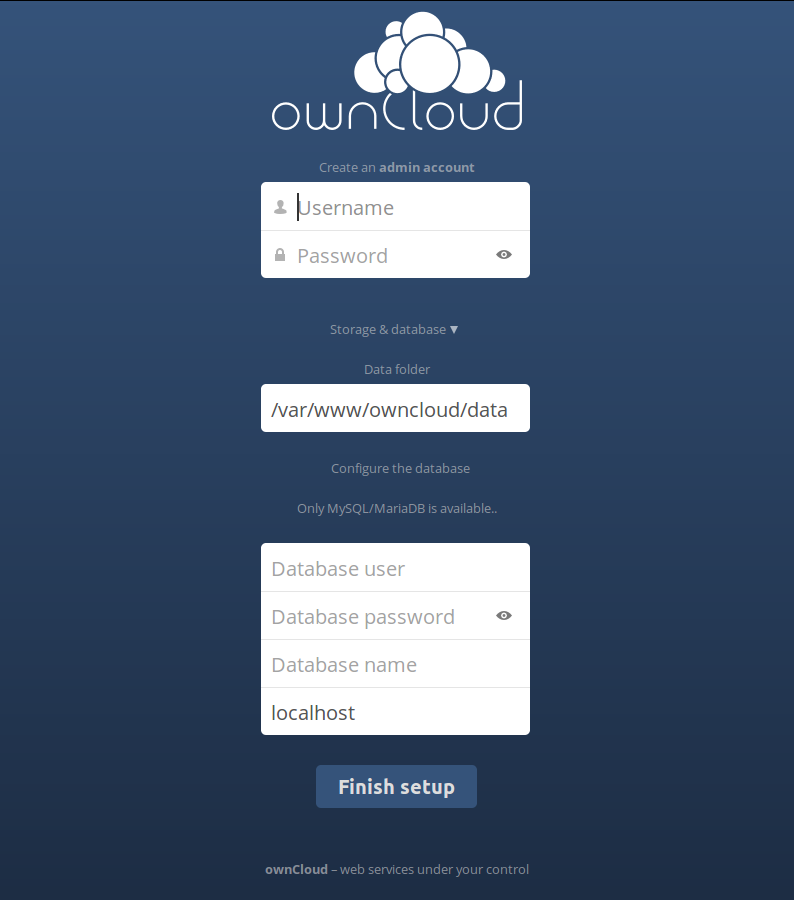
\includegraphics[width=0.8\linewidth]{img/OCWelcomePage.png}
  \caption{ownCloud - Page d'accueil}
  \label{ocwelcomepage}
\end{figure}

\clearpage
\section{Création du compte administrateur}

Sur cette page web, qui est l'administration du serveur ownCloud, il faut à présent créer un compte administrateur et configurer la base de données en entrant des identifiants que vous avez créé précédemment.

\vspace{0.4cm}

\noindent NB : Si un message d'erreur indique que vous ne pouvez pas écrire dans le dossier, il faut créer le dossier puis changer les droits d'écriture de ce celui-ci ainsi que l'attribuer à l'utilisateur 'www-data' pour que l'administration puisse y accéder : \\

\begin{lstlisting}[language=bash]
  cd /var/www
  sudo chmod 755 owncloud
  
  cd /var/www/owncloud
  sudo mkdir data
  sudo chmod 766 data

  sudo chown www-data:www-data -R /var/www/owncloud/data
\end{lstlisting}

Si tout fonctionne correctement, vous serez dirigé vers le dashboard de votre compte ownCloud fraîchement créé (figure \ref{ocdashboard}). On peut voir que deux dossiers et un fichier ont déjà été créés.

\begin{figure}[h]
  \centering
    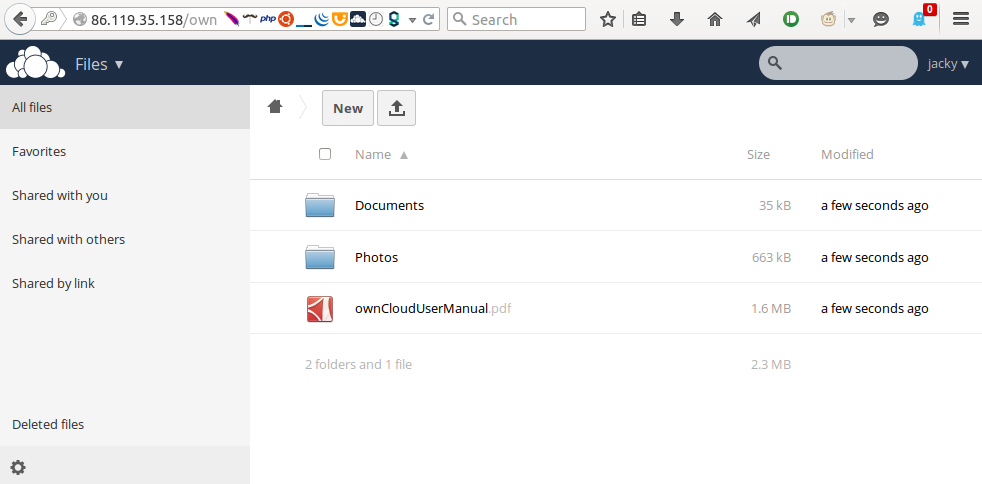
\includegraphics[width=\linewidth]{img/OCDashboard.png}
  \caption{ownCloud - Dashboard}
  \label{ocdashboard}
\end{figure}

\newpage

Vous êtes alors l'administrateur de ce serveur ownCloud. Vous pouvez gérer beaucoup de choses depuis l'interface de l'administration. Cette interface vous permet de gérer vos propres documents mais également de créer d'autres utilisateurs. Vous pouvez créer des groupes avec des droits spécifiques et mettre des utilisateurs dans ces groupes. Vous pouvez paramétrer des crons, paramétrer l'envoi d'emails, etc. 

Vos utilisateurs, ainsi que vous, pouvez installer un client ownCloud\footnote{Client desktop : \url{https://owncloud.com/products/desktop-clients/}} sur votre ordinateur (MacOX, Windows, Linux) pour synchroniser vos fichiers sur le serveur. Il existe également des application smartphone pour Android\footnote{Client Android : \url{https://play.google.com/store/apps/details?id=com.owncloud.android&hl=fr}} et iOS\footnote{Client iOS : \url{https://itunes.apple.com/fr/app/owncloud/id543672169?mt=8}}. Après l'installation, il suffit d'indiquer l'adresse du serveur, le nom d'utilisateur ainsi que le mot de passe et le tour est joué.\\

Ce guide d'installation d'un serveur ownCloud sur une instance SWITCHengines est terminé.

%\input{chapter/labo3.tex}
%\chapter{Conclusion}
%\section{Conclusion}



\vspace{3cm}
Fribourg, le \today

\vspace{1cm}

\hspace{11cm} Jacky \textsc{Casas}

\vspace{2cm}

%\newpage

%\appendix % annexes
%\chapter{Code source}
% \section{}


\end{document}
